% https://de.overleaf.com/learn/latex/How_to_Write_a_Thesis_in_LaTeX_(Part_1)%3A_Basic_Structure
% https://en.wikibooks.org/wiki/LaTeX/Document_Structure
%\documentclass[11pt, twoside]{report}
\documentclass[11pt, a4paper]{report}
%\documentclass[a4paper,11pt]{scrartcl}
\usepackage{syntonly}
%\syntaxonly
\usepackage[utf8]{inputenc}
\usepackage[backend=biber]{biblatex}
\addbibresource{mybib.bib}
\usepackage{hyperref}
\usepackage{graphicx}
\usepackage{color}
\usepackage{framed}
\usepackage{subcaption}
\usepackage{float}
\graphicspath{ {images/} }
\usepackage{blindtext}
\usepackage{mathtools}
\usepackage{amssymb}
\usepackage{amsfonts}
\usepackage{amsthm}
%\usepackage{showframe}
%\usepackage[a4paper, width=150mm, top=5mm, bottom=5mm]{geometry}
\usepackage[a4paper, width=150mm, top=25mm, bottom=25mm]{geometry}
\usepackage{fancyhdr}
%\setlength{\headheight}{12pt}
%\setlength{\headheight}{15.2pt}
%\pagestyle{empty}
%\pagestyle{myheadings}
%\pagestyle{headings}
%\pagestyle{plain}
\pagestyle{fancy}
\fancyhf{}
%\fancyhead[L]{\leftmark:}
%\fancyhead[L]{\chapter~\thechapter:}
%\fancyhead[L]{\thechapter}
\fancyhead[C]{\rightmark}
%\fancyhead[R]{\thesection}
\fancyfoot[C]{\thepage}

\setlength{\parskip}{1.0em}
\setlength{\parindent}{1em}

\usepackage{lipsum}

\theoremstyle{plain}
\newtheorem{theorem}{Theorem}[chapter]
\newtheorem{lemma}[theorem]{Lemma}

\theoremstyle{definition}
\newtheorem{mydef}{Definition}[chapter]

\theoremstyle{remark}
\newtheorem{remark}{Remark}[chapter]


%newcommands
\newcommand{\N}{\mathbb{N}}
\newcommand{\C}{\mathbb{C}}
\newcommand{\R}{\mathbb{R}}
\newcommand{\Z}{\mathbb{Z}}
\newcommand{\E}{\mathbf{E}}
\newcommand{\F}{\mathbb{F}}
%\newcommand{\B}{\{-1,1\}}
\newcommand{\bvec}[1]{\mathbf{#1}}
\newcommand{\bv}[1]{\mathbf{#1}}
\newcommand{\ceil}[1]{\lceil{#1}\rceil}
\newcommand{\floor}[1]{\lfloor{#1}\rfloor}
\newcommand{\gt}{>}
\newcommand{\lt}{<}
\newcommand{\tuple}[1]{\langle #1 \rangle}

\begin{document}
%\pagestyle{fancy}
\begin{titlepage}
\begin{center}
{
\includegraphics{images/MPIMG_RGB_gruen.png}}\\
\vspace*{1cm}
%\vfill
\Large
\textbf{List of topics to cover}
%\vfill

%\vspace{0.5cm}


%\normalsize
\large
With section titles and brief explantions.
\vfill
%\vspace{1.0cm}

Yiftach Kolb

Berlin, \today

\vfill
{
\includegraphics{images/fu-logo_bildschirm_RGB1.jpg}}
\end{center}
\end{titlepage}

%\author{Kolb, Yiftach}
%\date{Berlin, \today}
%\title{Topic List}
%\maketitle

\chapter*{Abstract}
punkt.
punkt.
\nocite{guo2017improved}

\chapter*{Declaration}
punkt.
punkt.
\nocite{bishop2006pattern}
\nocite{serre2001matrices}
\nocite{kingma2013auto}
\nocite{lotfollahi2018generative}

\chapter*{Acknowledgement}
punkt.\cite{kingma2013auto}
punkt.

\listoftables

\listoffigures

\tableofcontents

\chapter{Introduction}
punkt.
punkt.

\chapter{Autoencoders, VAEs, and Variance inference}

\section{Some basic definitions and concepts}
%\begin{mydef}
%\label{def:datamatrix}
A \textit{data matrix} is simply a real valued matrix $X \in \R^{N \times n}$
which represent a set of $N$ $n$-dimensional data points.
The $N$ rows are also called \textit{observations} and the $n$ columns are
\textit{variables}.
For example $X$ may represent $N$ cells over $n$ genes in the case of
single-cells RNAseq data.
%\end{mydef}

%\begin{mydef}
%\label{def:NN}
A \textit{feed forward neural network} is simply a differentiable map $\phi :
\R^n \to \R^m$.
Normally $\phi$ is a sequence of composition of some more simple functions which
we call \textit{layers}. A layer is composed of a single affine function,
followed by $0$ or more dimension preserving functions such as normalization
functions or activation functions. An activation function is a real values
non-linear function which is applied element-wise over the input later.
For example the sigmoid function anb the ReLU (rectified linear unit) are
probably the most well-known activation functions.

%\end{mydef}

Usually together with a neural network comes an associated differentiable
function which is the \textit{loss function} $\mathcal{L} : \R^m \to \R$.

The basic functions which comprise $\phi$ are parametrized. For example each
affine function has the form $f:x \to a\dot x + b$. $a$ and $b$ are its
trainable parameters, whereas the input is treated as fixed (the data we are
trying to explain). The set of parameters of $\phi$ (coming from all the
functions comprising it) is also referred to as its \textit{weights}. We can
therefore treat $\phi$ as a parametrized function $\phi_w$ where $w$ represents
the set of trainable weights.


Trining the neural network means finding the weights that minimize the loss function 
applied on the training set $X$, in other words minimizing 
$\min_{w} (\mathcal{L}(\phi_w(X))$.
During a training step the network is applied on a batch $X_k$ (a subset of size
$k \leq N$ of $X$, $X_k$ is therefore a $k\times n$ data matrix). 
Then the the loss function is applied at the output and a gradient
(with relation to the weights) is taken. This gradient is used for the wieght
update rule, which varies depending on the specific training algorithm (for
example SGD or Adam).



\section{Autoencoders}
An \textit{Autoencoder} (AE) is a neural network $\phi = D \circ E$ with a "bottleneck" layer which
approximates the identity function on the training input.
We call the part which maps the input into the bottleneck the \textit{encoder} and the
part which maps the bottleneck into the input-spce the \textit{decoder}.

A typical loss function for the AE is usually the mean sum of squares (MSE)
$\mathcal{L}(X;\phi) = \frac{1}{N}\|X - \phi(X)\|_F^2 = \frac{1}{N}\|X - D \circ
E (X) \|_F^2$.

Note that the MSE can be interpreted probabilitically, if we assume our input
comes from a random diagonal Gaussian with constant unit variant, we can interpret
$D(E(X)) = \mu_x$ and the mean square error is $\log \mathcal{N}(x ; mu_x, 1)$
(up to some scaling factor). Where $\log \mathcal{N}(\cdot ; \mu_x, 1)$ is the 
log-density function for diagonal Gaussian with mean $\mu_x$ and unit variance. 


\subsection{Relation between PCA and AE}
In fact, for centered data $X$ (every variable has $0$ sample mean), the first
$k \leq R(X)$ principle components $P$ are the soloution for 
$P = \text{argmin}_{W^T W = I_k} (\|X - XWW^T\|_F^2)$, whereas a linear autoencoder
solves $E,D = \text{argmin}_{E,D}(\|X - XED\|_F^2)$, and it can be shown than
it must hold that $E = D^{\dagger}$ (the encoder must be the Moore-Penrose
inverse of the decoder).

A linear autoencoder (an AE where $\phi$ is linear) is therefore almost equivalent to
PCA~\cite{plaut2018principal}, in that in the optimum, a bottleneck space of dimension $k$
is spanned by the first $k$ principle components of the input $X$.
In general, an AE can be seen a PCA-like, but non-linear method for
dimensionality resuction.

\section{Variational Inference}


Here we briefly explain the idea behind variational inference and introduce the
ELBO which is the loss function we'll use throughout this text.
For more details see~\fullcite{bishop2006pattern}.

We have a set of observation $X = \{x_1, \dots , x_N\}$ which we try to explain
by a probabilitic model. 
$X$ is called the data or the observation (or something similar). We assume that
the $x_i$'s are i.i.d with some distribution function $p(x)$ and therefore for
the entire dataset it holds that $p(X) = \prod x_i$.

We have some reason to believe that behind the scences there is some hidden
(latent) shot caller $Z = \{z_1 \dots z_N\}$ that determines the fate of $X$.
In other words we think that $X$ is conditioned on $Z$ and and we can speak of
the joint distribution $p(X,Z) = p(X|Z)p(Z)$ and all said distributions factor
over the individual samples multiplicatively, i.e.
$p(X|Z) = \prod p(z_i | x_i)$.

Suppose that we have a fully Bayesian model. In this case there are no
parameters because the parameters are themselves stochastic variables with some
suitable priors. We can therefore pack all the latent variables and stochastic
parameters into one latent "meta variable" $Z = (z_1, z_2, \dots )$, each $z_i$
is some multidimensional r.v and possibly composed of several simpler r.vs (for
example a categotical and a normal r.vs).
We similarly pack all the observed variables into one meta variable $X$.
Together we have a distribution $p(X,Z)$ and the working assumption is that it
is easy to factorize $p(X,Z) = p(X|Z)p(Z)$, however $p(Z|X)$ is intractable and
$p(X)$ is unknown.

We are being Bayesian here so we consider $X = (x_1, x_2, \dots)$ to really be
constant, a set of observation and we want to best explain $p(X)$ by finding as
high as possible lower boud (or rather to $\log p(X)$, the log evidence).
A second goal is to approximate the intractable $p(Z|X)$ by some simpler
distribution $q(Z)$ taken from some family of distributions.

The following equation finds a lower bound (elbo) for the log evidence.
(using Jensen's inequality)

\begin{equation}\label{eq:elbo}
\begin{aligned}
\log p(X) &= \log \int p(X,Z) dZ = \log \int \frac{p(X,Z)}{q(Z)} q(Z)dZ \\
&= \log \int \frac{p(X,Z)}{q(Z)}dq(Z) 
\geq \int \log \frac{p(X,Z)}{q(Z)}dq(Z) 
\triangleq \mathcal{L}(q)
\end{aligned}
\end{equation}

In equation~\ref{eq:elbo} we found a lower bound $\mathcal{L}(q)$ for the log
evidence $\log p(X)$, which we call "evidence lower bound" or elbo for short.
Whatever distribution $q$ we put in elbo will not be
greater than the real log evidence so we are looking for the $q$ which
maximizes it.

Now we show that maximizing actually obtains the log evidence and it is
equivalent to minimizing $KL(q(Z) \| p(Z|X)$:

\begin{equation}\label{eq:kl_bound}
\begin{aligned}
\mathcal{L}(q) &\triangleq \int \log \frac{p(X,Z)}{q(Z)} d q(Z)
= \int \log \frac{p(Z|X)p(X)}{q(Z)} d q(Z) \\
&= \int \log p(X) dq(Z) - \int \log \frac{q(Z)}{p(Z|X)} dq(Z) 
= \log p(X) - KL(q(Z) \| p(Z|X)
\end{aligned}
\end{equation}

We can rewrite equation~\ref{eq:kl_bound} as:
\begin{equation}\label{eq:elbokl}
\log p(X) = \mathcal{L}(q) - KL(q(Z) \| p(Z|X))
\end{equation}

Equation~\ref{eq:elbokl} shows the the elbo minus the kl-divergence are constant
and equal the log evidence. Therefore minimizing the kl-divergence (which is
always non-negative) simultaneously maximizes the elbo and vicer-versa.

\section{Adding parameters}

Our models will not be fully Bayesian, but rather parametrized.
In this case let $\theta$ represent the set of parameters for $p$, and $\phi$
the parameters for $q$. Meaning we are dealing with a family of distributions
$p_{\theta}(x,z)$ and another family $q_{\phi}(z)$.

For any $\theta$ and any $\phi$, the equations from the previous chapter hold
also in the parametrize form, i.e $\log p_{\theta}(x) = \mathcal{L}(q_{\phi}) -
KL(q_{\phi}(Z) \| p_{\theta}(Z|X)$.

We assume that we can only approach the "real" distribution using
$\theta$ from below $\log p(X) \geq \log p_{\theta}(X)$.
So together with equation~\ref{eq:elbo} we have

\begin{equation}\label{eq:parelbo}
\begin{aligned}
(\forall \theta, \phi)\log p(X) & \geq \log p_{\theta}(X) \geq \mathcal{L}(q_{\phi})
= \int \frac{p_{\theta}(Z|X)}{q_{\phi}(Z)} dq_{\phi}(Z)
\end{aligned}
\end{equation}

So from equation~\ref{eq:elbokl} we again see that by finding the parameters
$\phi$, $\theta$ that maximize the elbo we approach the real log evidence as much
as we can within the limits of the parametrized family of distributions we use.

\subsection{Using neural networks for the parametrization}
In this text we deal with variational autoencoders (VAE).
A VAE is a neural network which is used to define and optimize the parameters
$\phi$ and $\theta$.

Specifically the encoder part of the network is a non-linear map $f_{\theta}(Z)$ which is
used to define $P_{\theta}(X|Z)$. For example, we can assume that $P_{\theta}$
is a family of multivariate Gaussians and in this case $f_{\theta}(Z) =
(\mu(Z), \Sigma(Z))$. Meaning the encoder maps $Z$ to the location vector and
covariance matrice. The parameter $\theta$ in this case are the weights of the
encoder neural network. In parametrize the prior $p(Z)$ however in this case its
parameter is not a function of $X$. In practice there is no reason to do this
for most VAEs and we choose some simple fixed prior distribution for $p(Z)$.

The decoder network is similarly defined as a non-linear function $g_{\phi}(X)$ which
maps $X$ into the parameters defining the family $q_{\phi}(Z)$. Here too $\phi$
represent the weights of the decoder.

\remark{}\label{rem:abuse_of_notation}
In many papers about VAEs (including this text) the decoder is described as
$q_{\phi}(X | Z)$. This is an abuse of notation, because there is neither 
join distribution $q_{\phi}(X,Z)$ nor marginal $q_{\phi}(X)$ to speak of.
However $q_{\phi}(Z)$ is meant to approximate the intractable $p(Z|X)$ and
that's presumably the reason for the abused notation.


\section{Graphical representation}

%punkt.
%punkt.
%\remark{My remark}[See \cite{makhzani2015adversarial}] This is interesting
%\dots.
%punkt.

It is both convenient as well as informative to include a graphical description
of our probabilitic models by way of plate diagrams.

Please note that we drop the $\phi, \theta$ subscript but they are still there
in reality.

In a plate diagram nodes represent random variables and arrows
represent dependency.
Figure~\ref{fig:vae_model} is a plate diagram of the VAE model with slight
adaptation. We use doted arrows to represent the arrows of the inference model,
and regular arrows for the generative model. Regular (triangular) arrowhead
represents real probabilitic dependency whereas rounded arrows are reminding us
that this is not a real probabilitic dependency (recall
\ref{rem:abuse_of_notation}) which maybe we can call 'parametric
dependency'.

Plate represents packing of $N$ i.i.ds since we have $N$ observations $X =
(x_i)_1^N$ and correspondingly $N$ latent variables $Z = (z_i)$.

Shaded node represent known values (either observation of prior).

The squared $\zeta$ node represent some fixed parameters which describes the
prior distribution of $P(z)$. Usually it is not shown in the papers about VAE
but we just wanted to remind the reader that it can be parametrize in general.

The generative model therefore factors as: $p(x,z) = p(x|z)p(z|\zeta) =
p(x|z)p(z)$

The inference model in this case is just $q(z)$ but we might denote is as
$q(z|x)$ because it tries to approximate $p(z|x)$.

Note that the graphical model has no assumption about the specific types of
distributions involved (Gaussian, Dirichlet or whateve \dots) and that is left
for the actual implementation.

In the case of a "vanilla" VAE, We chose the prior to be diagonal standard Gaussian
$p(z) \sim N(;0,1)$. And $p(z | x)$ is then chosed as diagonal Gaussian (whose
means and variances we find by training the network).

\begin{figure}
\centering
\begin{subfigure}[b]{0.2\textwidth}
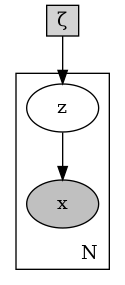
\includegraphics[width=\textwidth]{../plots/vae_p.gv.png}
\caption{generative model ($p(x,z)$}
%\caption{blabla}
%\label{bla}
\end{subfigure}
%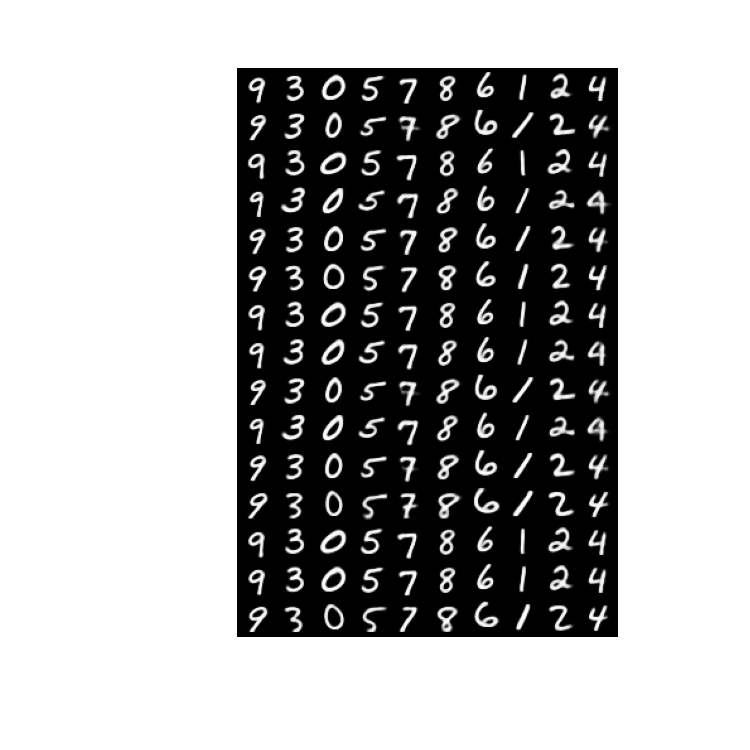
\includegraphics[width=0.4\linewidth]{images/model_mnist_10c_generation.png}
\begin{subfigure}[b]{0.2\textwidth}
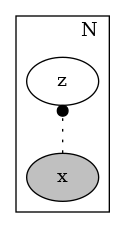
\includegraphics[width=\textwidth]{../plots/vae_q.gv.png}
\caption{inference model ($q(z|x)$)}
%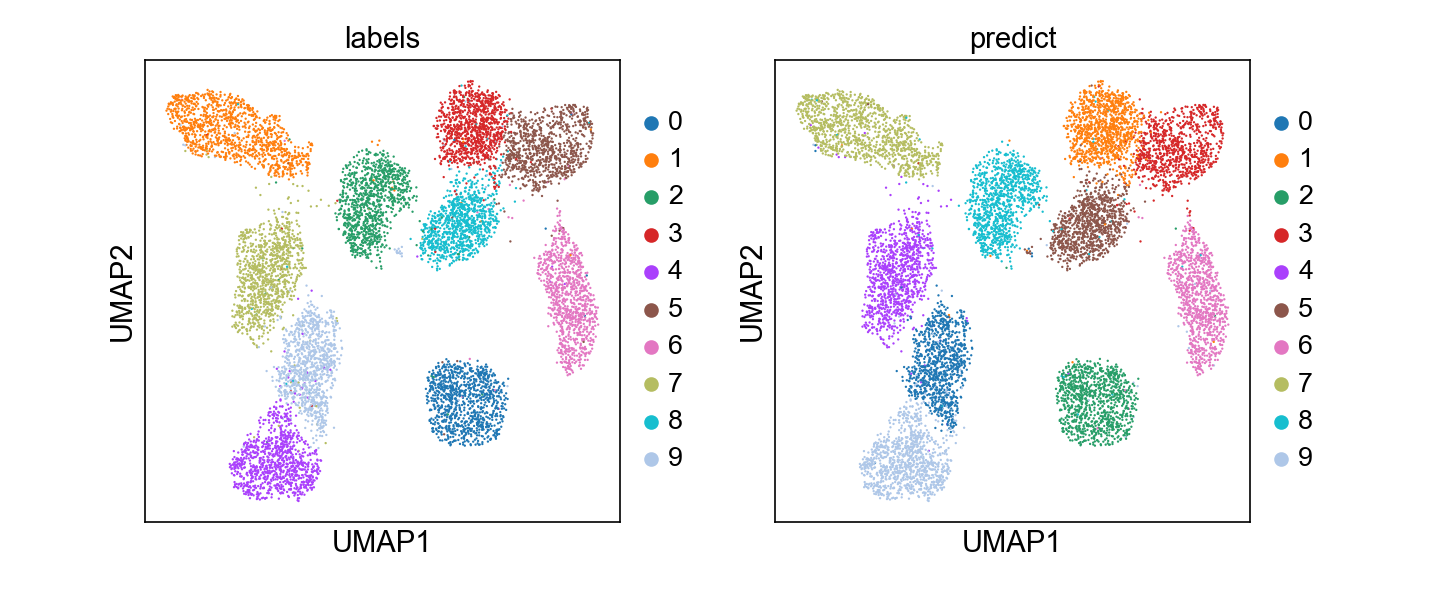
\includegraphics[width=0.4\linewidth]{images/model_mnist_10c_umap.png}
\end{subfigure}
\begin{subfigure}[b]{0.2\textwidth}
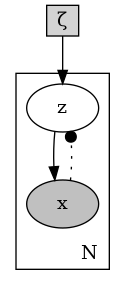
\includegraphics[width=\textwidth]{../plots/vae.gv.png}
\caption{the combined graphical model}
%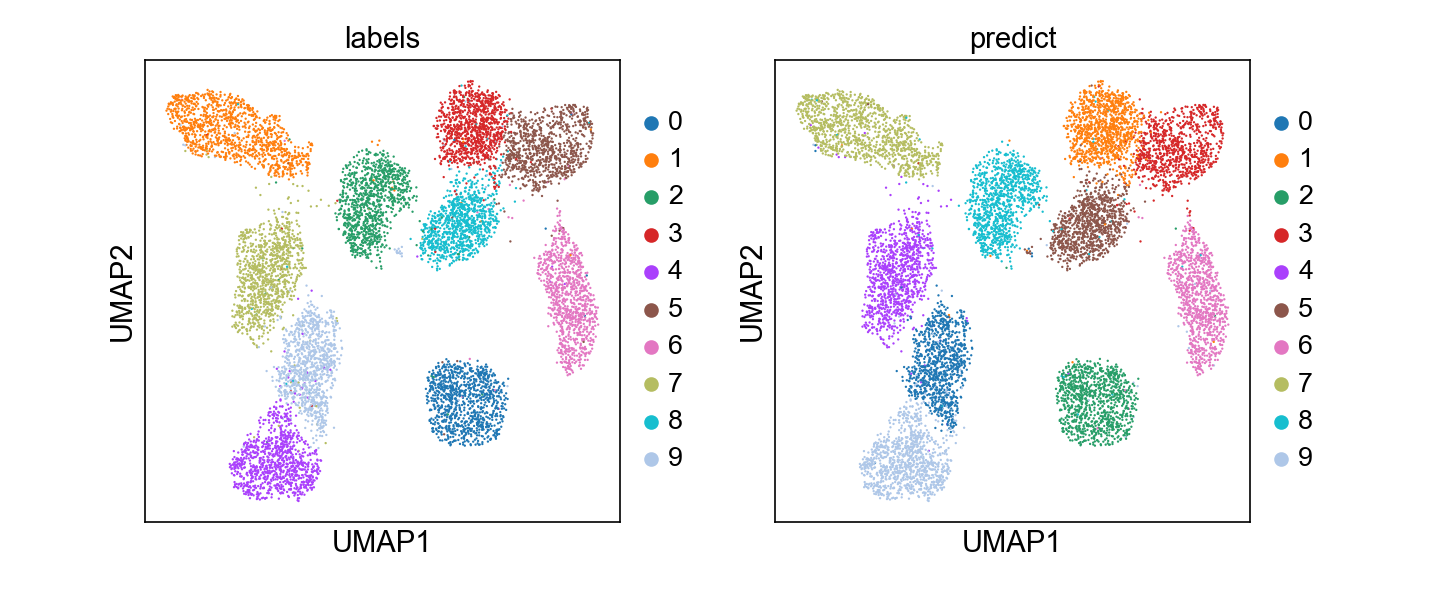
\includegraphics[width=0.4\linewidth]{images/model_mnist_10c_umap.png}
\end{subfigure}
\caption{VAE graphical model}
\label{fig:vae_model}
\end{figure}

\chapter{Gaussian mixture model VAEs}

Theoretical background and 
with some examples from publications and my own tests.


\begin{figure}
\centering
\begin{subfigure}[b]{0.4\textwidth}
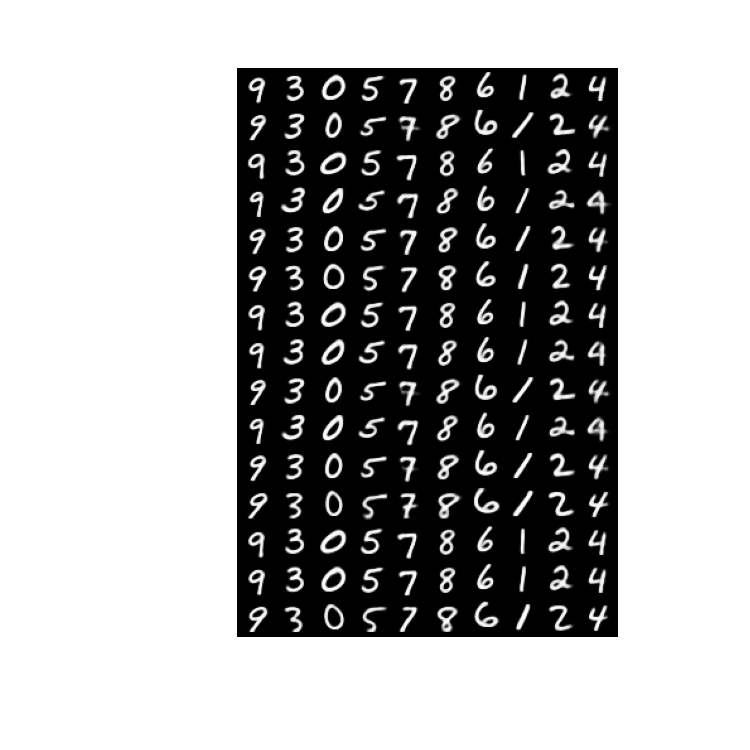
\includegraphics[width=\textwidth]{images/model_mnist_10c_generation.png}
\caption{}
%\caption{blabla}
%\label{bla}
\end{subfigure}
%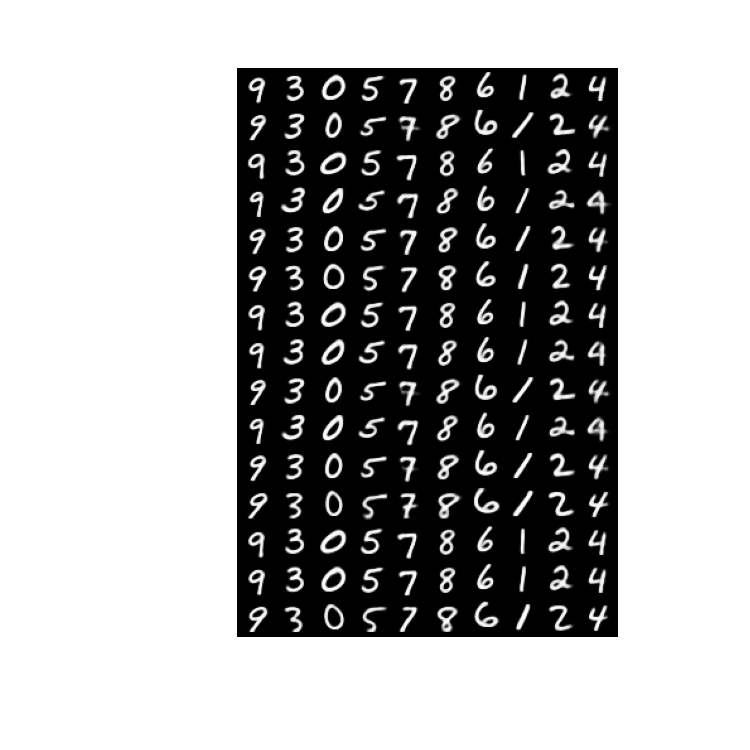
\includegraphics[width=0.4\linewidth]{images/model_mnist_10c_generation.png}
\begin{subfigure}[b]{0.4\textwidth}
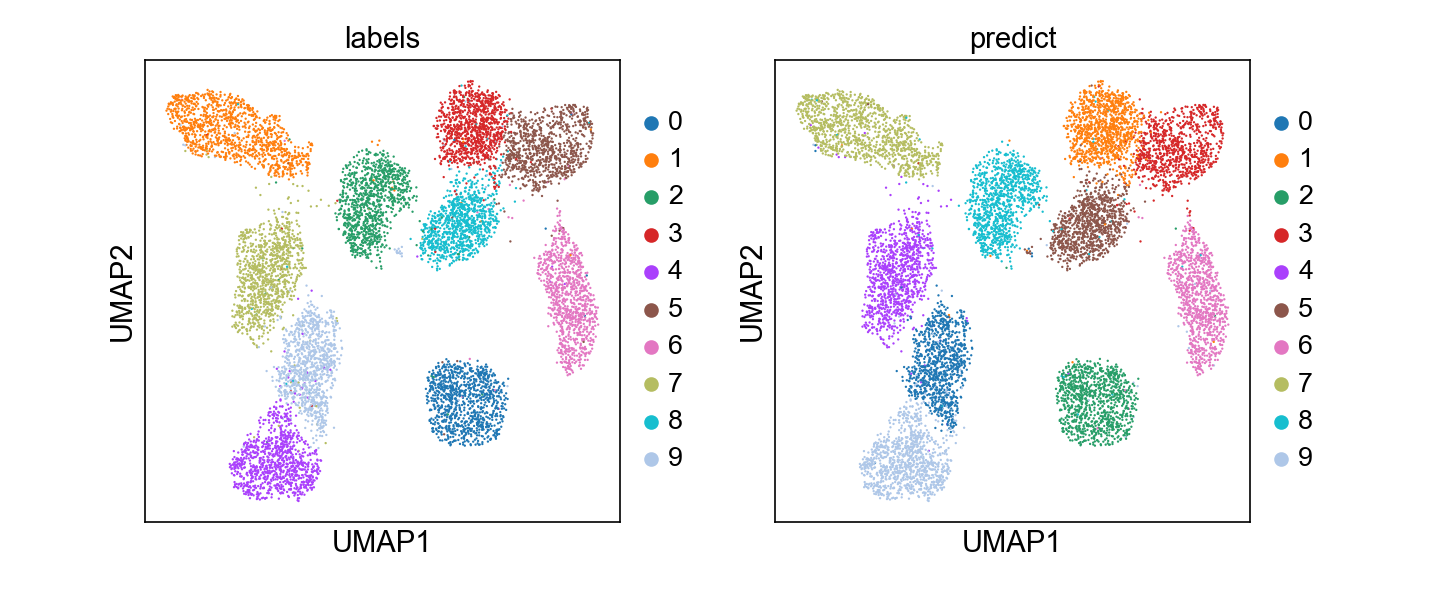
\includegraphics[width=\textwidth]{images/model_mnist_10c_umap.png}
\caption{}
%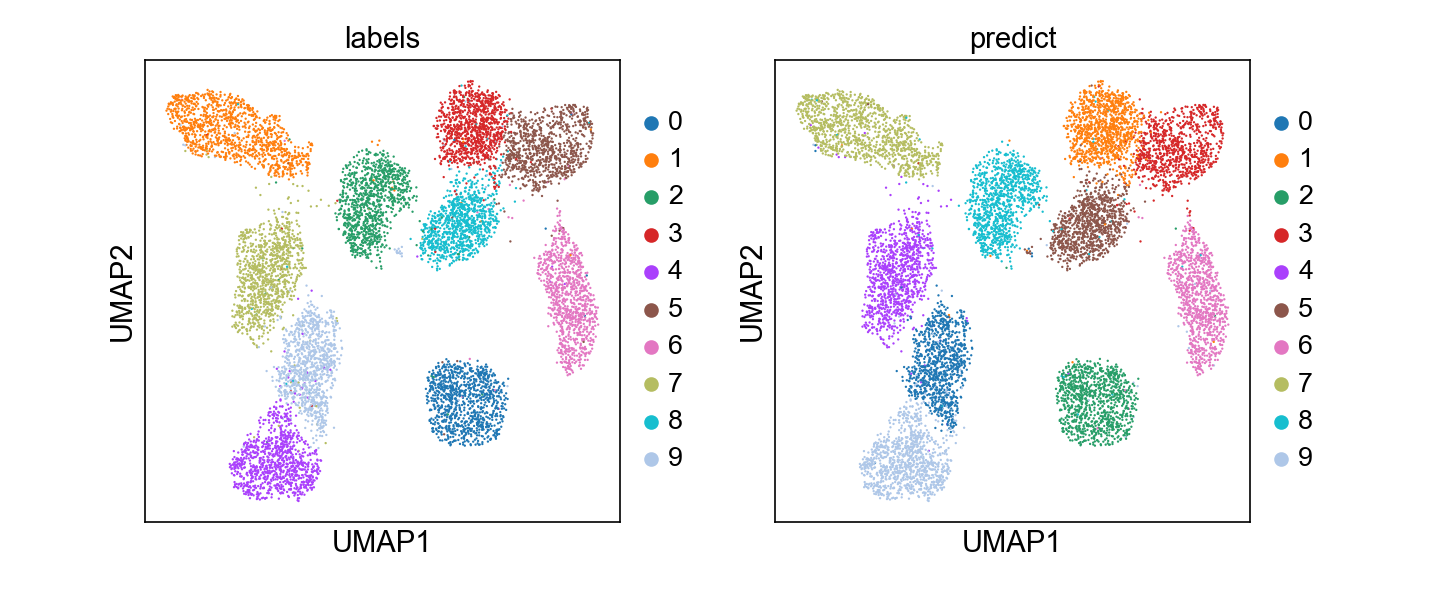
\includegraphics[width=0.4\linewidth]{images/model_mnist_10c_umap.png}
\end{subfigure}
\caption{a figure}
\label{fig:myfig}
\end{figure}

\chapter{Datasets which were tested and results}
some words about (sc)RNAseq and published papers where 
AE and VAE models have been applied.
What we were hoping to achieve and compare with.

\chapter{Discussion, some remarks and conclusions}
punkt.
punkt.
punkt.





%\author{Yiftach Kolb}
%\date{Berlin, \today}
%\maketitle

%\section*{Intro Foo}
%\lipsum{1}
%\section{Bar}
%\lipsum{2}
%\appendix
%\section{Spam}
%\lipsum{3}

\printbibliography

\end{document}


